
%%% Local Variables:
%%% mode: latex
%%% TeX-master: t
%%% End:

\chapter{概述}

\section{背景} 
深圳市交通仿真系统(二期)构建了“ 1+2+2”的体系, 包括一个可动态更
新的多元交通、土地利用大数据平台, 以及专题数据挖掘分析系统、交通与土地
利用一体化交通模型系统、综合交通信息分析查询系统和面向多用户模型应用系
统四个子系统。\fref{fig:项目体系架构}是整个项目的体系架构图。

\begin{figure}[!hbt]
  \centering
  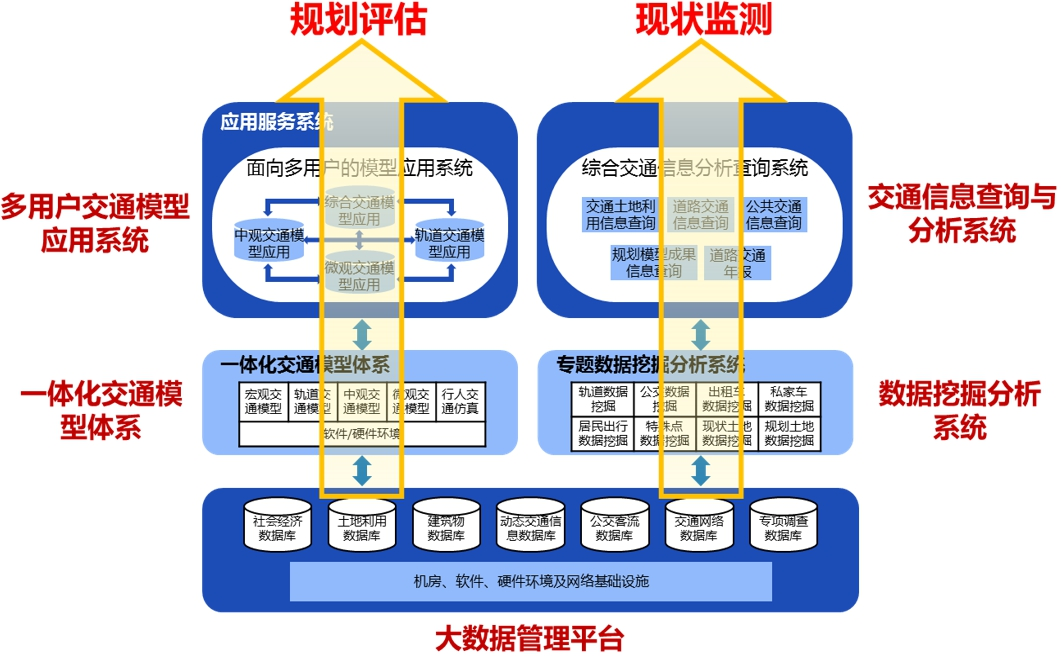
\includegraphics[width=\textwidth]{figures/chp01_项目体系架构.jpg}
  \caption{深圳市交通仿真系统(二期)的“ 1+2+2”体系\label{fig:项目体系架构}}
\end{figure}

其中, 深圳市交通仿真系统(二期) 项目已完成的工作包括:

\begin{para}
\item[多元数据平台] 负责对全市智能交通系统采集的动态交通数据、人口岗
位等社会经济数据以及土地利用、城市规划等 GIS 数据进行集中管理。
截止项目验收,数据更新至 2013 年 12 月;
\item[一体化交通模型体系] 全市宏观交通模型、罗湖区中观交通模型和大剧
院、大运会区域微观交通仿真模型和香蜜湖地铁站行人仿真模型;
\item[专题数据挖掘分析系统] 用于对多元数据平台的各类型数据按照交通和
土地利用指标进行挖掘分析,分析结果同样更新至 2013 年 12 月;
\item[面向多用户模型应用系统] 将一体化模型中的容积率、用地功能能重要
参数以接口形式提供出来, 由规划人员按照规划方案设定相关参数进行
模型运算,用以简化模型使用的难度;
\item[综合交通信息分析查询系统] 将专题数据挖掘分析系统中挖掘计算的各
类指标推送至浏览器前端,提供用户进行成果查询和展示的功能。
\end{para}

但是,在深圳市快速发展的背景下,为了能够更好地反映交通的特征和变化
趋势,以及构建快速响应的交通仿真模型,对深圳市交通仿真系统(二期)原有
数据和已建成系统的更新工作具有十分重要的意义。

因此,从 2015 年开始,将系统日常更新列为年度常规性工作。在原有系统
的基础上,主要针对 \pyear 年交通情况从底层数据平台到上层模型和信息化系统
进行统一的更新。一方面,通过系统的数据分析结果反映最新的现状交通特征,
并且可以通过与之前年份的数据进行对比,发现城市交通运行的变化趋势;另一
方面,通过更新工作,对原有模型系统进行补充和完善,提高原有模型精度,扩
大模型建设范围,为未来的交通规划工作提供定量依据和决策支撑。

\section{项目内容}
本项目延续了深圳市交通仿真系统(二期)“ 1+2+2” 的体系结构,更新的工
作主要包括数据更新、 信息化系统更新和模型更新三块内容。 其中,数据更新、
信息化系统更新在原有系统基础上, 按照深圳市交通仿真系统(二期) 系统设计
的更新技术要求进行常规类作业; 模型更新除在原有一体化模型体系基础上进行
常规性数据更新之外,还按照原有模型体系和建模技术要求, 新建福田区中观模
型和两个重点区域微观模型。 具体的工作可以分解为以下几个部分:

\smalltitle{数据更新}
在\pyear 年各类型动态交通数据和静态 GIS 数据基础上,采用人工编辑和自
动化处理相结合的技术方法对原始数据进行加工和处理,使其符合深圳市交通仿
真系统(二期) 中多元数据平台的入库要求,将原有系统中的数据扩充至 \pyear
年。

\smalltitle{数据挖掘系统更新}
在数据更新的基础上,采用自动化程序对\pyear 年各类交通指标数据进行重
新挖掘分析,在原有数据基础上扩充\pyear 年指标数据, 并将更新后的挖掘指标
推送至数据查询系统。

\smalltitle{宏观模型更新}
宏观模型更新的主要内容包括更新输入条件以及模型优化两方面。输入条件
更新包括综合网络更新、人口及土地利用数据、轨道OD矩阵更新等。模型优化的工作包括
收入模型、拥车模型和发生吸引模型。

\smalltitle{新建盐田、大鹏中观交通模型}
新建盐田区和大鹏新区中观交通模型,包括现状年模型和规划年模型。主要内容包括:
宏观模型截取区域路网及矩阵、小区及交通需求矩阵拆分、现场交通量调查、
模型校核、规划年路网更新、规划年需求矩阵预测、规划年新增用地交通需求叠加等工作。

\smalltitle{重点片区微观模型建设}
近年来,在城市轨道交通详细规划和交通枢纽改善规划等项目中,对交通枢纽建立行人微观仿真模型的
需求越来越多。因此,本项目基于行人仿真技术,新建大运枢纽规划行人仿真模型和高新园地铁站现状
行人仿真模型。

\smalltitle{数据查询系统更新}
在数据挖掘推送的指标数据基础上,采用自动化程序更新系统后台数据库,
并且在系统的前端将涉及到更新的功能展示出来, 使用户可以查询到 \pyear 年更
新的全部指标数据。

\smalltitle{数据查询系统更新}
在数据挖掘推送的指标数据基础上,采用自动化程序更新系统后台数据库,
并且在系统的前端将涉及到更新的功能展示出来, 使用户可以查询到 \pyear 年更
新的全部指标数据。

\smalltitle{系统运维}
针对深圳市交通仿真系统(二期) \pyear 年运行中出现的系统问题和异常进
行处理和维护, 并且在系统更新完成后进行年度的系统备份,保证系统的稳定运
行和异常恢复。

\section{技术路线}
\subsection{数据和信息化系统更新}
数据更新、数据挖掘系统更新和数据查询系统更新是承上启下的串行工作路
线,严格按照图中的流程进行作业, 但是每一部分内容内部又可以细分为并行流
程和串行流程; 相比前几项工作, 系统运维工作比较独立,备份工作需要在其他
所有工作完成后开展, 而其他两项工作可以在系统测试、 运行和使用的过程中同
步开展。\fref{fig:数据和信息化更新技术路线}是数据和信息化系统更新的技术路线图。

\begin{figure}[ht]
  \centering
  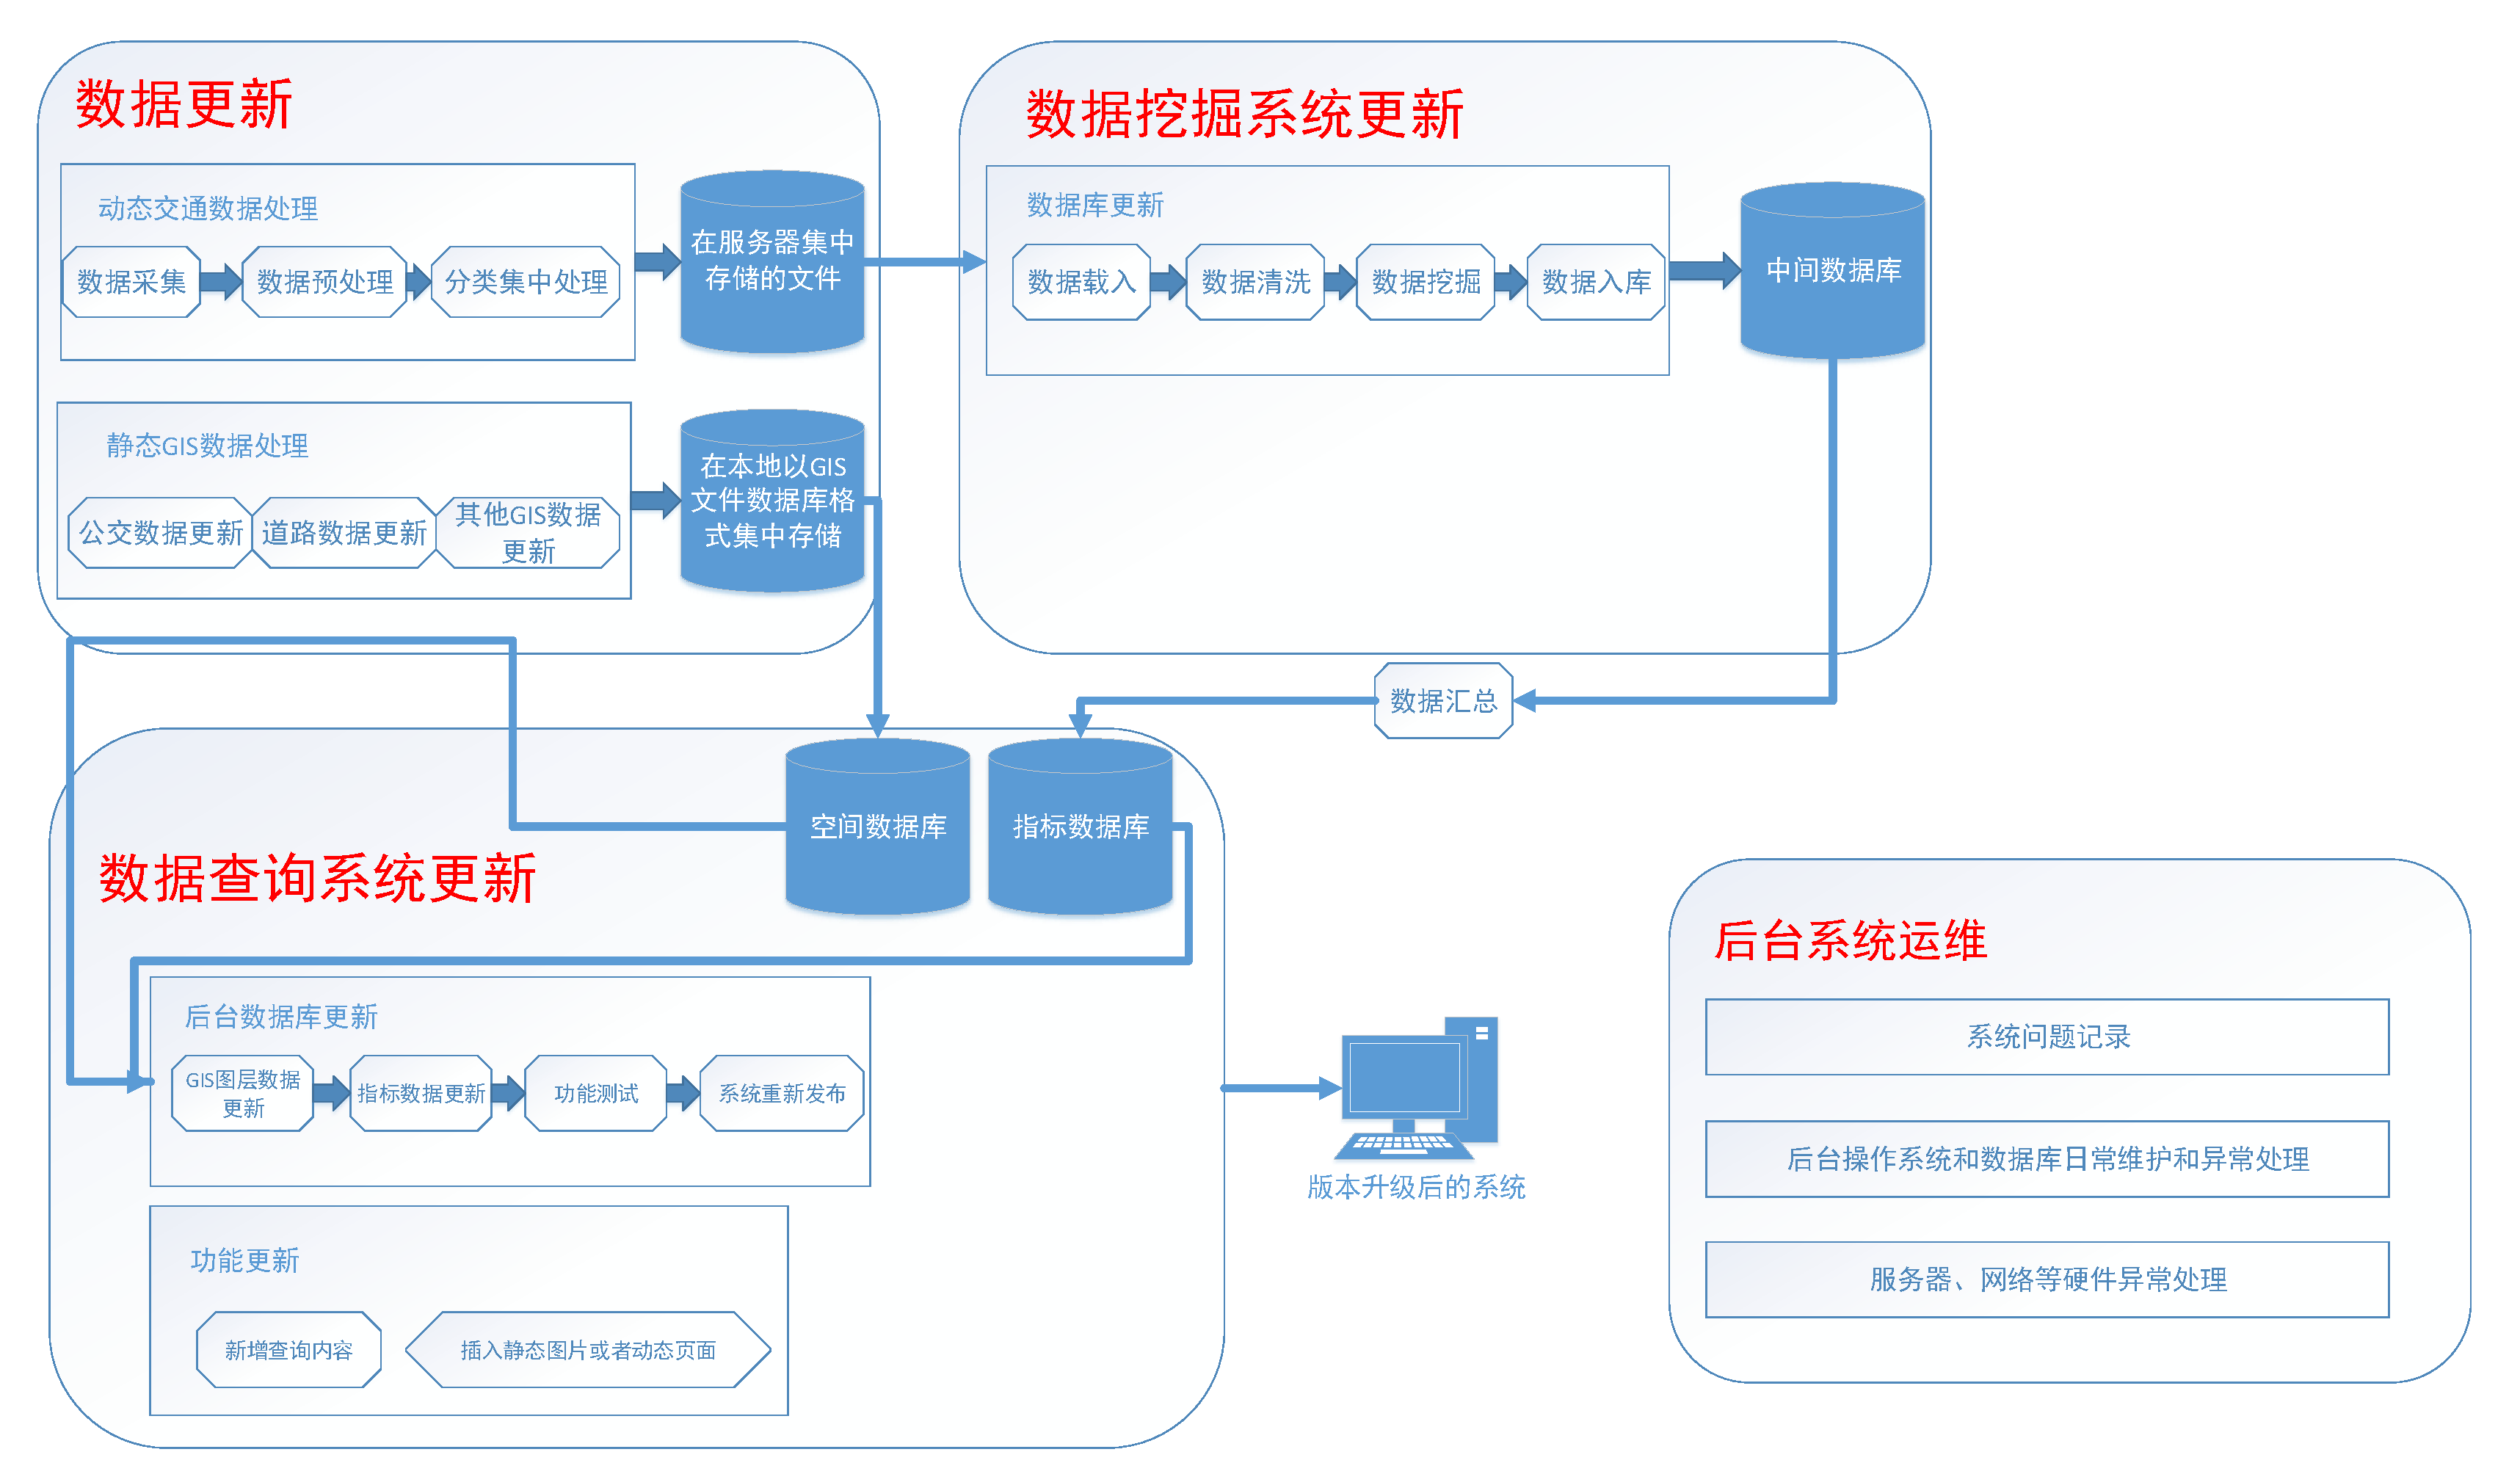
\includegraphics[width=\textwidth]{figures/chp01_数据和信息化更新技术路线.pdf}
  \caption{数据和信息化系统更新技术路线\label{fig:数据和信息化更新技术路线} }
\end{figure}

\subsection{交通模型更新}
在数据更新的基础上, 项目对深圳市交通仿真系统(二期) 已建成的全市宏
观模型进行数据更新和参数更新等工作, 保证模型中的现状年模型输入数据为最
新的交通数据。 按照深圳市交通仿真系统(二期) 设计的一体化模型体系建模思
想和技术路线, 采用德国 PTV 公司的 VISUM 和 VISSIM 软件, 从已建成宏观模型
中通过子路网切割技术,继承了宏观模型交通需求和交通网络等基础数据,并对
交通小区、交叉口等路网信息细化,新建盐田区和大鹏新区中观模型;再由宏观交通模型分
配结果,自动导出用于枢纽行人微观仿真建模的人流量数据,新建重要交通枢纽
行人微观仿真模型。\fref{fig:一体化模型系统更新技术路线}是一体化模型系统更新的技术路线图。

\begin{figure}[ht]
  \centering
  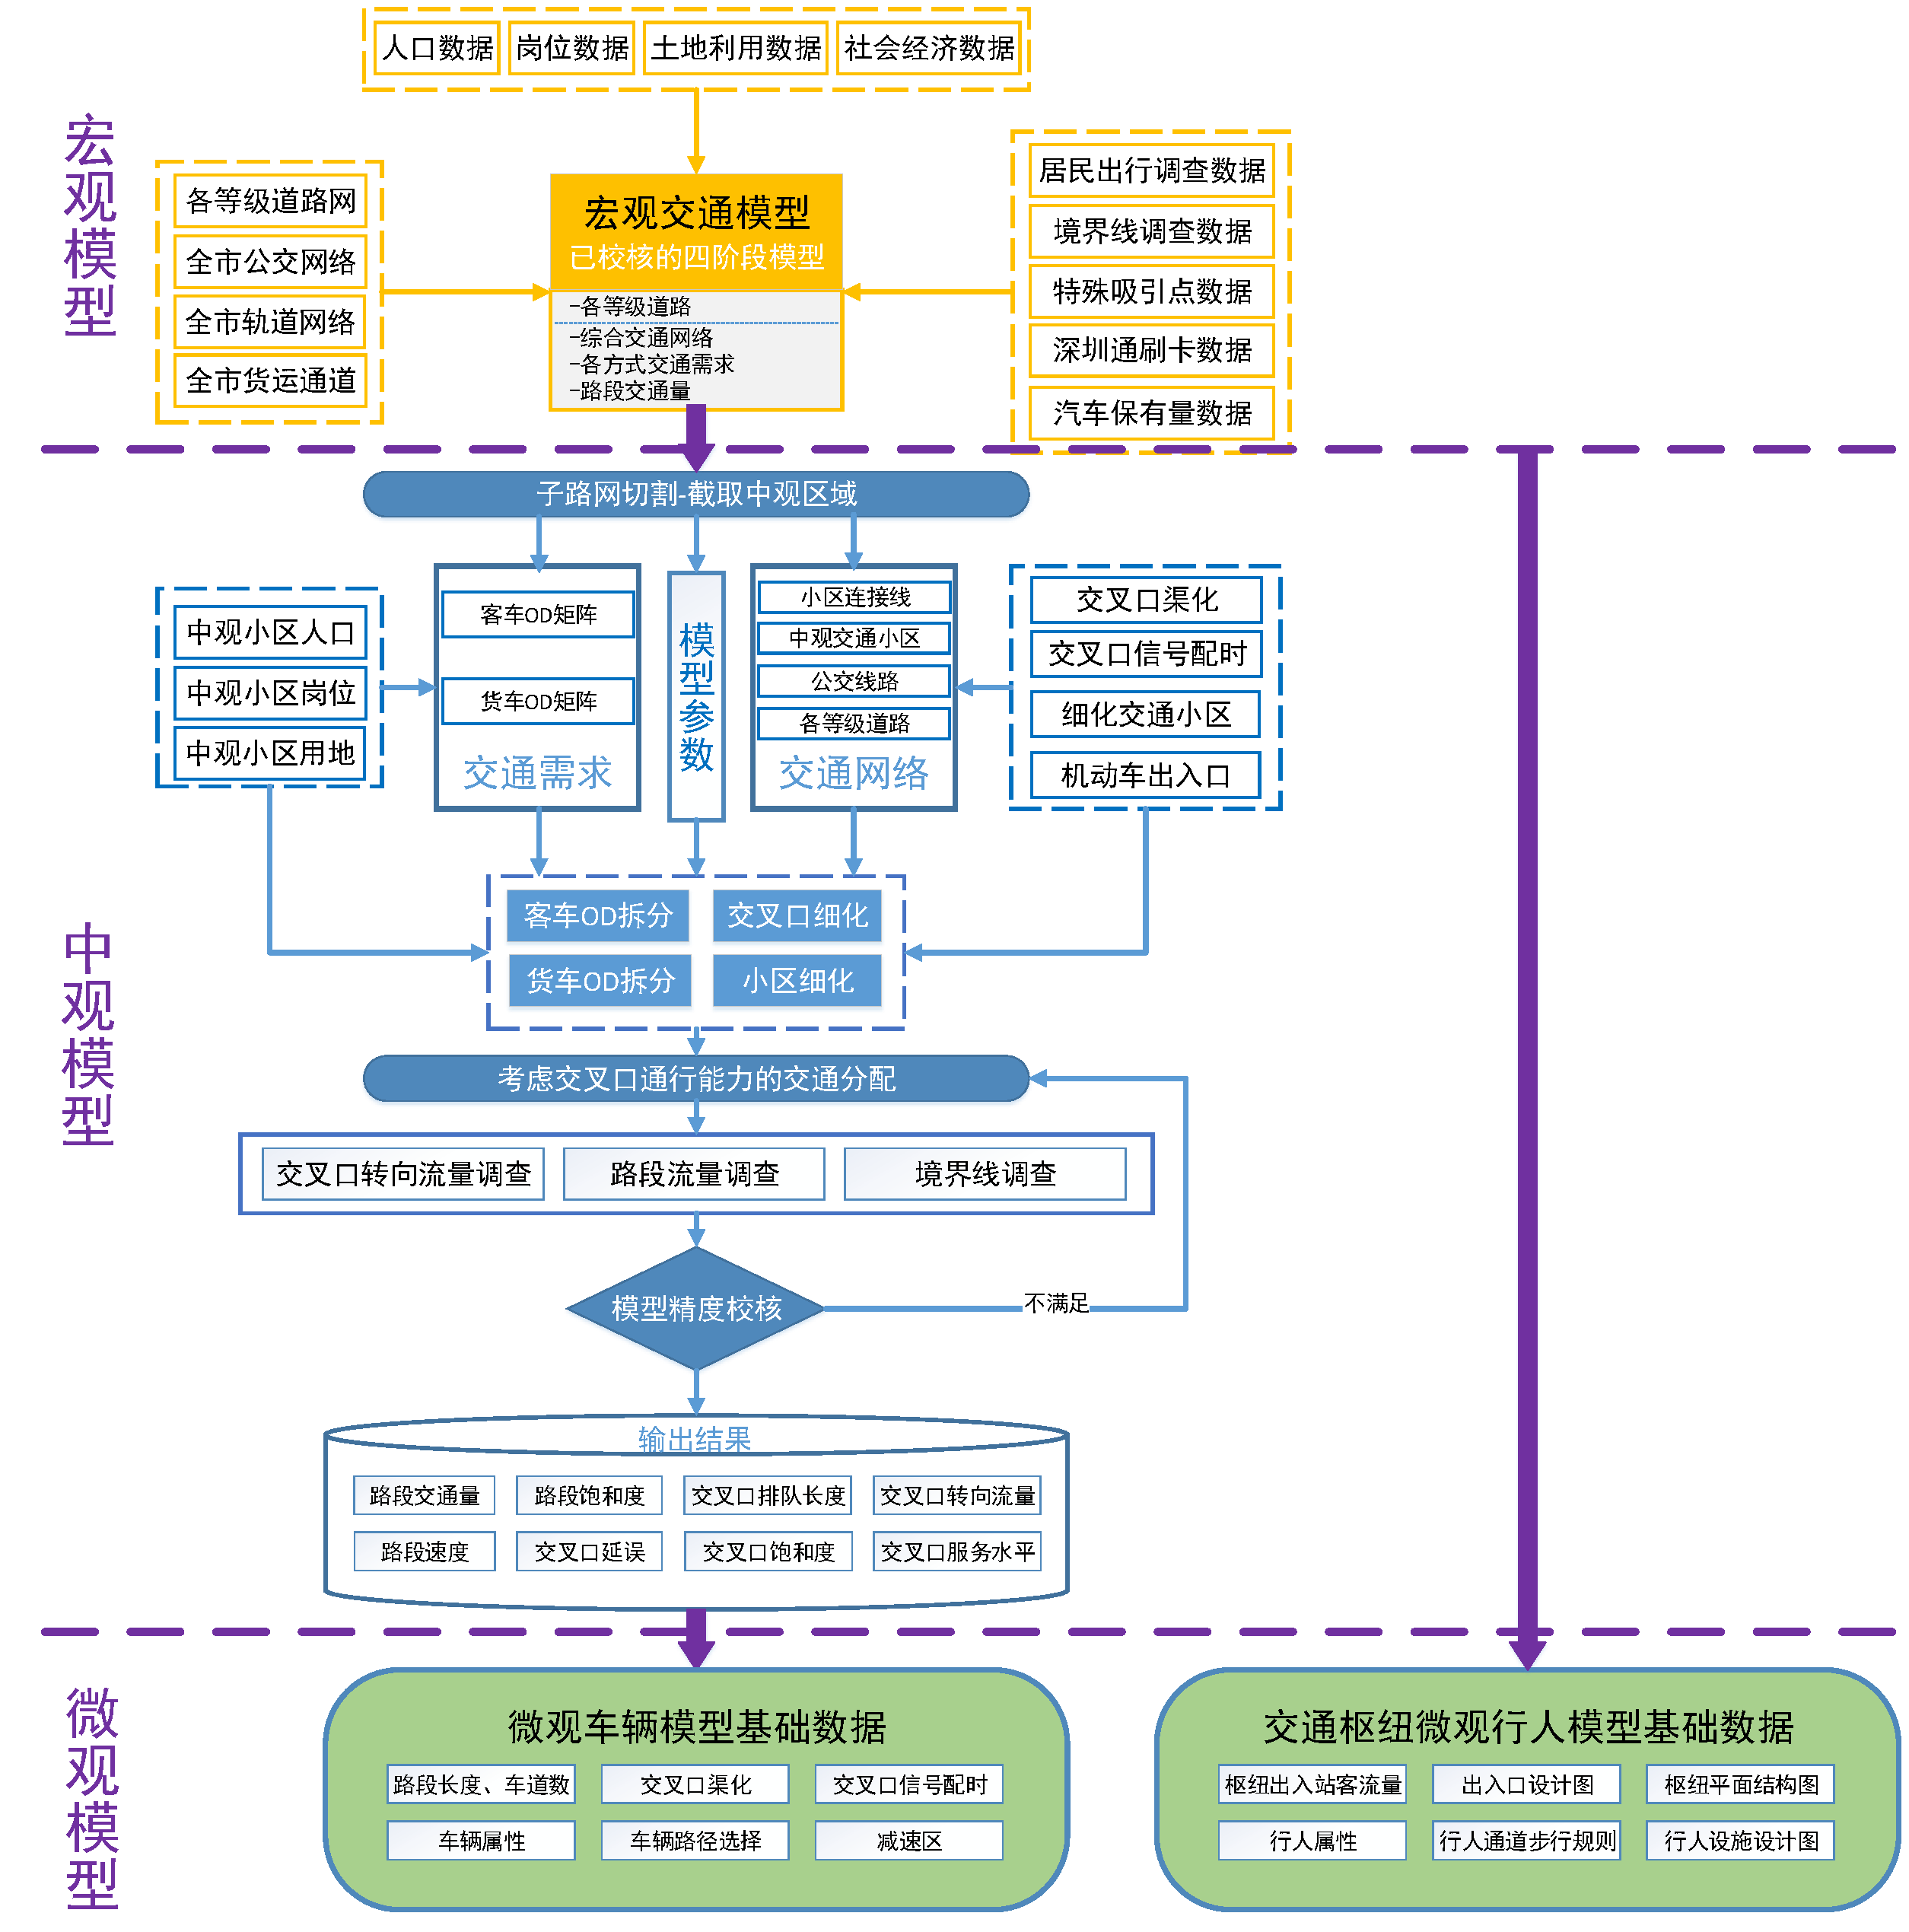
\includegraphics[width=\textwidth]{figures/chp01_一体化模型系统更新技术路线.pdf}
  \caption{一体化模型系统更新技术路线\label{fig:一体化模型系统更新技术路线} }
\end{figure}















